
\graphicspath{ {./figuras/model_performance/} }
\center
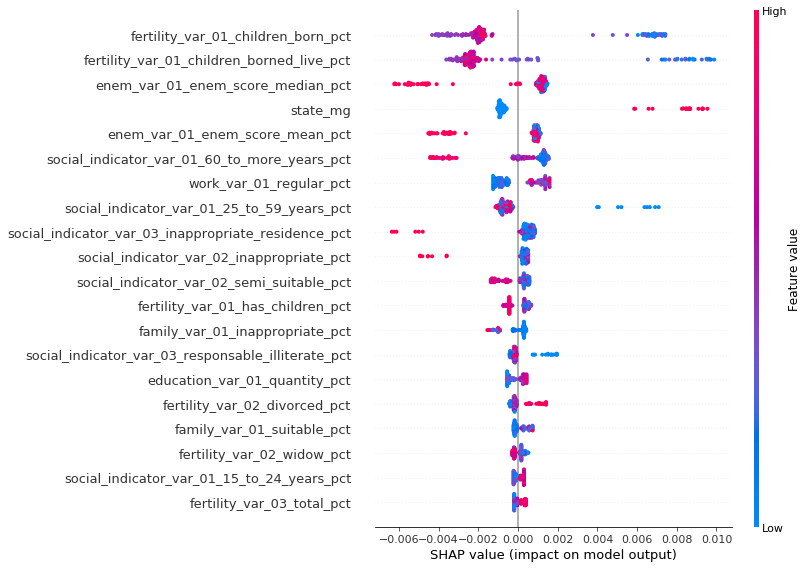
\includegraphics[width=14.0cm, keepaspectratio]{cap3_shap_random_forest}

\captionof{figure}{Shapley value do Random Forest}

\label{ape:cap3_shap_random_forest}




% \begin{figure}
%  \center
%   \includegraphics[width=\linewidth]{figures/figure_path.png}
%   \caption{Coloque label aqui}
%   \label{graph}
% \end{figure}

% \begin{algorithm}
% \caption{Least Squares - Single Node Localization}\label{LS_pseudocode}
% \begin{algorithmic}[1]
% \Function{Localization\_LS}{$\hat{\bm{P}}$, $\bm{d}_m\left(\bm{x}, \bm{P}\right)$, $\hat{\bm{x}}_{0}$, $\epsilon$}
% \BState \emph{Initialization}:
% \State $\hat{\bm{x}}_{k}  = \hat{\bm{x}}_{0}$
% \BState \emph{Loop}:
% \Repeat  
% \State compute $\bm{d}_p\left(\hat{\bm{x}_k}, \hat{\bm{P}}\right)$ using \eqref{eq:distance_calculation_vector}
% %
% \State compute $\bm{H}_k$ using \eqref{eq:H_matrix}
% %
% \State compute $\hat{\bm{x}}_{k+1}$ using \eqref{eq:iterative_algo}
% \Until $\left|\left|\hat{\bm{x}}_{k+1} - \hat{\bm{x}}_{k}\right|\right| < \epsilon$\\
% \Return$ \hat{\bm{x}}_{k+1}$
% \EndFunction
% \end{algorithmic}
% \end{algorithm}